\section{Fault injection approach}\label{sec:approach}

%The approach we present in this paper 
\approach{} uses fault injection at run-time to test distributed embedded systems with very limited computation power. 
%Chaos Monkey Testing~\cite{FaaS,gunawi2011failure} and the Let-it-Crash paradigm~\cite{woskowskiassessing} are important related works, however, as mentioned before and further discussed in Section~\ref{sec:relatedWorks}, the characteristics of our target systems hamper their use in this context. 
Section~\ref{sec:researchMeth} presents the adopted research methodology, and Section~\ref{sec:approach_approach} presents an overview of the \approach{} approach. 

%This work has been developed in collaboration with a team within Ericsson AB in Gothenburg, Sweden. %\pat{add more details about the team within Ericsson}
%Due to the complexity of distributed systems and the challenges of testing distributed systems with traditional approaches, a new approach based on some existing distributed systems testing technique and researches is needed. %The main investigation of this thesis is how to develop a new fault injection approach and implement a new fault injection tool to help the development team at Ericsson in testing their embedded distributed system. Moreover, we aim to make the fault injection approach as general as possible so it can be used in other companies and bring benefits to the embedded industry in general.
%\newline
%As anticipated in the introduction t

\subsection{Research methodology}\label{sec:researchMeth}

Our collaboration model between academia and industry is based on the 
design and creation methodology, which was developed to address theoretical questions about the nature of learning
in context. It is mainly used when a creation of new knowledge is seeking in
order to solve a particular phenomenon through designing innovative artifact~\cite{ResMethod}.

The \approach{} approach and tool have been conceived and implemented following an agile development process %iteratively in four iterations 
and in strong synergy with practitioners within Ericsson. 
As anticipated in the introduction the approach and tool have been developed in four iterations and each iteration was composed of four phases, namely: 
\begin{itemize}
\item{\em Awareness of problem}: %collecting information about different fault types through deep literature studying. By studying the previous related work, we took an inspiration for developing the new approach. Furthermore, 
%basically through 
we had weekly 
meetings with practitioners %the supervisors 
at Ericsson and we analysed available documentation about the PM framework 
%organized by our industrial author 
%in order to gather more information on how the system works as well as some suggestions about the injection. We also analyzed Ericsson PM framework documents 
for identifying the bottleneck of the system and determining the injections. Additionally, Ericsson's internal fault reports and other available documents helped in gathering more information about the weakness of the system and identifying where problems can occur. 
%After deep studying of system weakness together with possible faults which might happen in reality, random faults were designed. At the same time the system was experimented by running with different scenarios and inspecting the log files. 
\item 
{\em Suggestion and solution}: based on Ericsson fault report and designed fault tolerant ability of the PM framework, potential fault types were discussed with practitioners. We decided to have two fault types, the first one was sending random messages and the second one was delaying messages. The rational of sending random messages is to 
%, we got the idea from the supervisor in order to 
test the filter ability of the PM framework against random invalid messages. Delaying the messages were performed between the critical components of the PM framework where faults can occur.
\item 
{\em Implementation}: the implementation contains two steps: tool development and tool integration. The first step mainly concerns the work of development the fault injection tool using an Ericsson internal shared library called Inter Process Communication. The second step mainly concerns the work of integrating the developed tool into the automatic testing environment of the PM framework.
\item 
{\em Evaluation}: since we followed an agile development process we had a continuous evaluation of the approach and tool through these means: %
%\begin{itemize}
%    \item 
(i) we had weekly meeting with practitioners for getting feedback;
    %\item Well identified requirements for the expected conformance level on how the tool should work.
%    \item 
(ii) continuous validation of  defined requirements for the expected conformance level on how the approach should work; 
%    \item 
(iii) observation of the results of the execution of the fault injection tool stored in log files;
(iv) comparison of the observed results with the expected ones (how the system should perform in its normal state);
%    \item 
(v) if faults were detected, evaluation of the faults by tracing back to the cause that made them.
%\end{itemize}  
\end{itemize}

\subsection{The \approach{} approach}\label{sec:approach_approach}

\begin{figure}[h]
\begin{center}
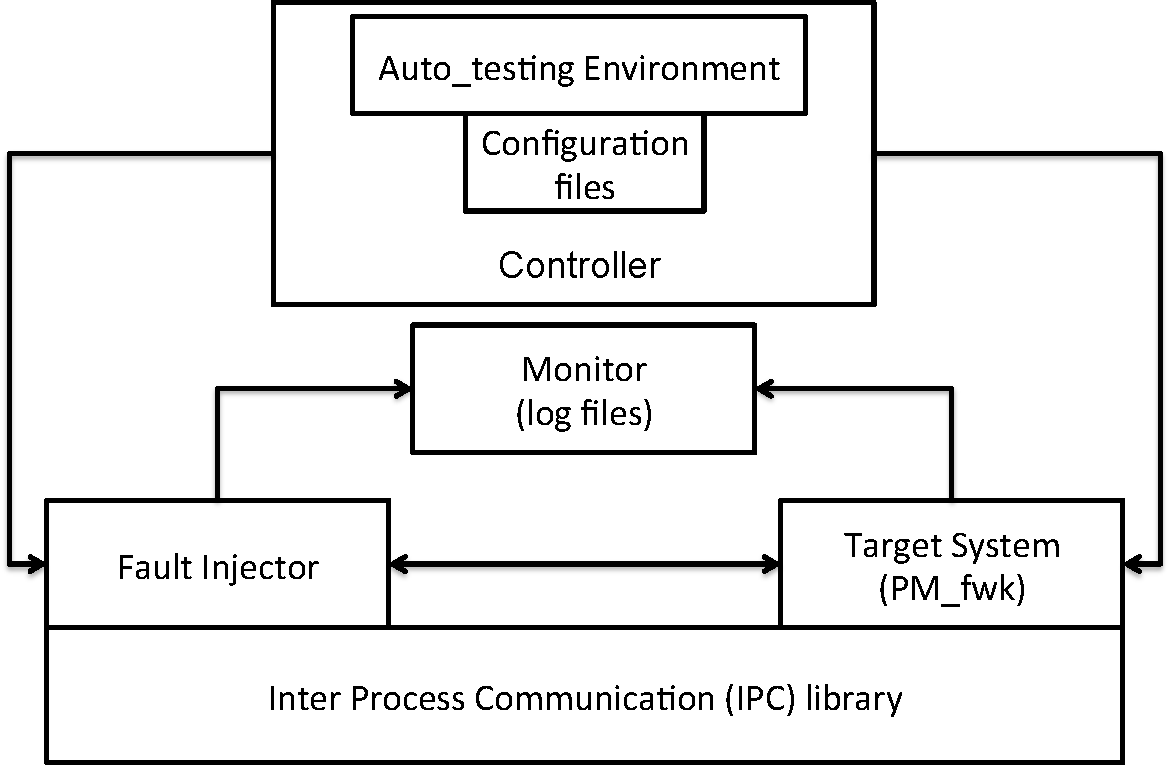
\includegraphics[width=\columnwidth]{figure/faultInjectionApproach.pdf}
\caption{The \approach{} approach \label{Fualt_injection_Model}}
\end{center}
\end{figure}

Figure~\ref{Fualt_injection_Model} presents the basic components of \approach{}. It consists of the target system (PM\_fwk), fault injector, monitor (log files), Inter Process Communication (IPC) library as well as the controller that has the automatic testing and the configuration files.
As better explained in Section~\ref{sec:implementation} configuration files are exploited to make the fault injector customizable, extensible, and reusable in different contexts.

After running the \approach{} tool all data are monitored from the log files using stack trace. These data are collected and analyzed for the evaluation of the approach and of the tool. % as well as for answering the main research questions. 
The user can run and control the tool through the controller, where the automatic testing environments and the configuration files are located. Through the automatic testing environment different testing techniques are listed. The \approach{} tool supports random mechanisms where the number of faulty messages, message delay, and the time interval between sending the messages are randomized. The user can manually adjust the test cases through the configuration files.    

The \approach{} approach provides different fault types at different location and time. We have developed two fault types: (i) sending random messages and (ii) delaying the messages. Fault types such as sending invalid messages and delaying the messages were done by linking some dynamic libraries of IPC during run time. IPC library is a separate component, which consists of different system functionalities such as sending the messages between different system component. After deep study of the PM framework documentation and discussion with the practitioners, system targets were identified. The system targets were some critical components of the PM framework that have strong dependencies. Faults were injected on system targets that have strong coupling. Due to the fact that time factor can have an effect on running the experiments and to make sure that the result we got are reliable, we have repeated the experiments at different time. For non deterministic testing, as pointed in~\cite{testselectionnondeterministic}, as long as the number of the repetition of test sequence increases, the quality of testing will also be increased. %In actual testing this number is limited due to economical and practical reasons. However, when executing the testing large number of time, the probability that all possible execution paths are executed will be reasonably high.  

\subsubsection{Sending random messages}
The communication within the system follows some specific protocols.  Sending random messages is mainly developed to test the fault tolerance ability of the protocols. The messages are categorized into three types: request, confirmation, and rejection.  Based on the designed fault tolerance feature and the possible message types in reality, we only perform sending of random request messages. We focus on three aspects of the invalid messages, the origination, the contents and the amount of sending.

The system is designed to tolerate invalid request messages, one main filtering standard of invalid messages is the origination of the messages. We focused on three aspects of the message origination, the namespace name, the mailbox name and combination of namespace and mailbox names. We first created multiple mailboxes which have the same namespace name, this means that the random messages are generated from different threads but the same process. Then we created mailboxes with same mailbox names but different namespace names; this means that the random messages are generated from both different threads and processes. Lastly, we created mailboxes with both different mailbox names and namespace names. Three cases of mailbox and namespace names are shown in Table~\ref{table:4.1}.

\begin{table}[ht!]
\centering
\begin{tabular}{| c | c | c |r}
 \cline{1-3}
       & mailbox & namespace \\ 
 \cline{1-3}
 case 1 & S & D & \hspace{1.3cm} S stands for same\\ 
 \cline{1-3}
 case 2 & D & S & D stands for different\\ 
 \cline{1-3}
 case 3 & D & D & \\ 
 \cline{1-3}
\end{tabular}
\caption{Combinations of mailbox and namespace names} %, S means same, D means different}
\label{table:4.1}
\end{table}

The message contents inside the system varied dramatically: some contents describe the actual payload, some describe the protocol version, some specify the size of the messages. The fields of the messages were also different from each other. Based on the above characteristics, we constructed the random messages from two different aspects, random fields and random contents. 

The amount of random messages would affect the filtering ability of the protocols. For instance, by sending one random message, the system is able to filter it, but by sending 1000 random messages, the system might only be able to filter 500 of them. With a huge amount of random messages, the CPU load of the systems would be high. 

\subsubsection{Delaying messages}
The second fault injection scenario was delaying the messages between the system components. The delay mechanism used default and randomize time interval between different components on the system in order to check if the system can handle different timeout intervals. There are multiple types of messages sending within the PM framework, e.g., request message, response message, rejection, confirmation message and messages describing the data. Some types of messages followed some time out mechanism strictly. For instance, when the connection request is sent, the node waits for confirmation or rejection messages for a period of time; if neither a confirmation nor a rejection message is received, the current request of the node just goes in timeout. 

\begin{figure}[hh!]
\centering
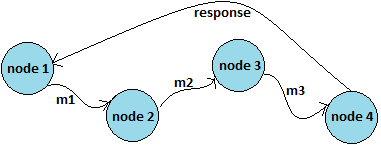
\includegraphics[width=.7\columnwidth]{figure/chaningMSG.png}
\caption{Message delaying chain \label{chaning}}
\end{figure}

Some messages sent within the PM framework have relationships with each other. Those messages usually work as a chain, as shown in Figure~\ref{chaning}. In this case, \texttt{node1} sends a request to \texttt{node4} for some data, and at the same time a clock starts for the time out mechanism. In order to receive the data, some messages are sent to \texttt{node2} and \texttt{node3}, but \texttt{node1} only waits for a response from \texttt{node4}. Delaying can happen on any of the messages sent between \texttt{node1} and \texttt{node4}. In reality, such a chain can be really long and the delay of the messages sent between each nodes can also be very unpredictable.

Delaying messages in the PM framework also tests the network performance of the framework. %By delaying messages in the PM framework, the network performance of the PM framework is tested. 
Currently the PM framework network performance test is conducted by adjusting the network bandwidth. This approach has two main drawbacks. First, the test has some hardware requirements, which makes the test more complicated. Second, adjusting the network bandwidth makes the test uncontrolled, because the delaying of the message caused by a low network bandwidth is very hard to track. The current network performance test is like a black-box testing, since what is really going on in the system during the test is not peered. Our test provides a white box testing for the PM framework network performance. During the message delaying, each message delaying is recorded in the log file, and then the PM framework developers at Ericsson can easily track the message delaying. A future network bandwidth benchmark has been created based on the experiences of the message delaying.


\section{Implementation}\label{sec:implementation}

The implementation consists of two steps: tool development and tool integration. The first step mainly concerns the development of the fault injection tool using an Ericsson internal shared library called Inter Process Communication (see Section~\ref{sec:IPC}); the results of this step are some compiled C++ object files. The second step mainly concerns the work of integrating the developed tool into the automatic testing environment of the PM framework, where Shell Scripts and Ruby were used (see Section~\ref{sec:PM}). Then, this section will describe the implementation of the procedure for the two fault types we considered in the study: sending random messages (see Section~\ref{sec:sendingRandomMessages}) and delaying messages (see Section~\ref{sec:delayingMessages}).

\subsection{Inter Process Communication}\label{sec:IPC}
Inter Process Communication (IPC) is used as a communication paradigm in some components of the PM framework. Collection of information from the system is done by handling the collection of the counters and events between its components. %\cite{pmf}.
 IPC is used to send messages between mailboxes, processes, and processors. A processor is an execution unit that is handled by one instance of an operating system, it can have multiple cores and several simultaneously executing contexts. A process has its own memory map and can have several running threads. A thread is a single execution context that can coexist with other threads within a process. We worked on a simulated environment, where the processor was the CPU of the computer, a process was a simulation of a processor on the embedded components,  and a thread was a simulation of a process in the real operating system. Figure~\ref{simulationVSembedded} shows the relationship between the real operating system and the simulated environment. In our implementation, only processes and threads were involved, they were identified by the process namespace and the thread name. %Both the namespace and the thread name have human readable names.
%\newline

\begin{figure}[h]
\centering
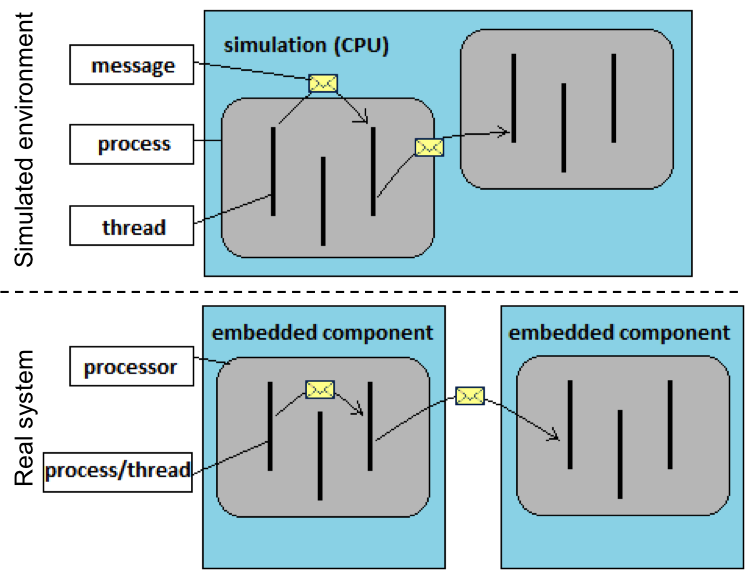
\includegraphics[width=\columnwidth]{figure/simulationVSembedded.png}
\caption{Relationship between real system and  simulated environment \label{simulationVSembedded}}
\end{figure}

IPC is a widely used library of RBS. The PM framework is built on top of IPC, it uses the APIs of IPC for the communication within the system. Based on this feature, we started our implementation without touching the code of the PM framework; instead we used the IPC APIs. In this way, we are able to inject random faults into the PM framework from outside the framework, and therefore that there is no need of extra computation for the framework to cater for fault injection. %This is a key difference with respect to Chaos Monkey Testing.

\subsection{Automatic testing environment}\label{sec:PM}
We developed a set of automated scenarios %that test the PM use cases that operation in reality
%In order 
to test the functions of the PM framework %, a set of automated scenarios that test the PM use cases that operation 
when operating in reality. % have been developed. 
The automatic testing environment is used to test the PM framework with such scenarios. The automated test scenarios will be used by the fault injection tool to verify that the PM works even in the presence of faults. 
%\newline

The \approach{} tool was integrated into the automatic testing environment using Shell Scripts, which injects random faults into the PM framework while running with the scenarios. The automatic testing environment also controls the operations of the fault injection tool like code generation, compiling and linking. The integration of \approach{} with  the automatic testing environment enhances the adoptability in industry and the usability of the tool.

%By integrating the tool into the automatic testing environment, the operation of the fault injection tool is more user-friendly and errors are more likely to be detected. 

The running results of fault injection are presented in the end of the automatic testing environment and traced in different log files. Figure~\ref{terminal} shows one type of running results in the end of the automatic testing environment, where the errors and corresponding log files are presented.
%\newpage

\begin{figure}[!ht]
\centering
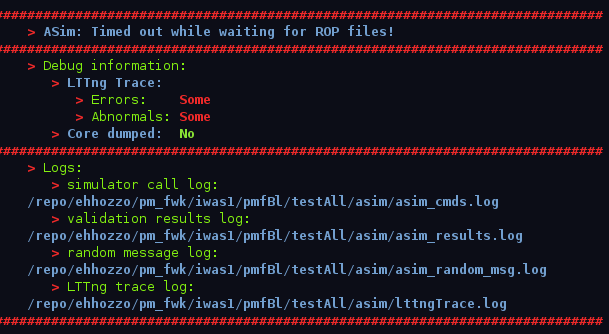
\includegraphics[width=\columnwidth]{figure/terminal.PNG}
\caption{Running results of automatic testing environment \label{terminal}}
\end{figure}


\subsection{Sending random messages}\label{sec:sendingRandomMessages}
In IPC, different messages were constructed with C++ structs; after initialization, the message objects were encapsulated in a message union and sent together. The fields of the messages are specified in some XML files; an excerpt is shown in Listing~\ref{xml_code}. We first ignored those files and constructed the messages with random fields, this means that the messages might miss some necessary fields and might contain some extra unnecessary fields. After that we constructed the messages following the XML files but with randomly filled contents, for instance, making the field called messages size to be a random number instead of the real message struct.         
%\newline                                              

\begin{minipage}{.96\columnwidth}
\lstinputlisting[
    language=xml,
    firstline=1,
    lastline=4,
    firstnumber=1,
    caption={XML that specifies message fields},
    label={xml_code},
]
{code/xml.xml}
\end{minipage}

Constructing the message structs was based on the skeleton of the XML files, different categories of messages had different message fields and required different C++ header files. In order to implement the randomization mechanism, all the request message structs and their corresponding required header files need to be considered. %The existing request messages might change in the future. 
To make the functionality of sending random messages customizable, 
%, to make the messages which were to be sent controllable, 
the message are specified in a configuration file. A code generator written in Ruby is used to create the message structs. By reading the configuration file and the XML file that specifies the message fields, different message structs code are generated and compiled to different binaries. 
%\newline

The next step after the construction of random messages is %being constructed, the next step was 
to create the senders. The senders are actually some mailboxes located in the same namespace, which means that each mailbox has a separate thread and they are all located in the same process. In order to send the messages to some targets, the mailbox address of the targets should be known. In the PM framework, the mailbox addresses can be located by using combinations of the namespace names and the mailbox names. In our implementation, we put all the namespace names and mailbox names into vectors, we calculate 
%tried to locate 
all possible combinations and we put them into a map.  %as shown in Listing~\ref{locate_code}. 
So if there are $n$ namespace names and $m$ mailbox names, then we have $m*n$ combinations in total. Once a TID\footnote{TID stands for Thread ID, i.e. an identifier used to identify a thread. It is also used to identify the mailbox associated with that thread.} is successfully located, it is saved in another vector which will be used as the target to send. The messages are sent in two different ways, synchronously and asynchronously. Sending the messages synchronously is  implemented by joining the mailbox to the main thread.  
%\newline

%\begin{minipage}{.96\columnwidth}
%\lstinputlisting[
%    language=C++,
%    firstline=1,
%    lastline=9,
%    firstnumber=1,
%    caption={Code that creates all combinations of namespaces and mailboxes},
%    label={locate_code},
%]
%{code/code2.cc}
%\end{minipage}

Sending random messages is integrated into the automatic testing environment, which is written in Shell script. Every error triggered by the random messages is logged and the logging is implemented with a watch dog. The watch dog keeps track of which message are sent and how many of them were sent. The watch dog also keeps pinging all the previously located TIDs and if any of them crashes during the time when the messages are sent, the watch dog would also log such a TID. The log file provides a summary of all the relevant events happened while injecting random messages to the PM framework; this facilitates the detection of errors that are not found with unit testing.

\subsection{Delaying messages}\label{sec:delayingMessages}
The message sending of the PM framework uses IPC by linking some dynamic libraries during run time. In C and C++, it is possible to wrap the dynamic library functions. Such a wrapping is implemented by creating shared libraries that override the functions of the original dynamic libraries. Such a dynamic library file can be linked by setting an environment variable called \texttt{LD\_PRELOAD}. We implemented the delaying messages by wrapping the IPC dynamic libraries that are responsible for sending messages. As shown in Listing~\ref{wrap_code}, the name of original message sending function was called  \texttt{\_\_itc\_send}, the main parameters of this function were the message contents named ``{\em msg}", the receiver named ``{\em to}" and the sender named ``{\em from}". The wrap function had exactly the same function name and parameters with the original function. 
%\newline

\begin{minipage}{.96\columnwidth}
\lstinputlisting[
    language=C++,
    firstline=1,
    lastline=16,
    firstnumber=1,
    caption={Code that wraps the sending function of IPC},
    label={wrap_code},
]
{code/code.cc}
\end{minipage}


%At Line 13, a function called ``{\em dlsym}" took a handle of the dynamic library which contains the \texttt{\_\_itc\_send} function, this handle was returned to a function pointer called \texttt{\_\_real\_itc\_send}, which has the same parameter types as the original \texttt{\_\_itc\_send} function. By calling the \texttt{\_\_real\_itc\_send} function with the original parameters of \texttt{\_\_itc\_send}, the original \texttt{\_\_itc\_send} got called. But 
As can be seen in Line 14,
before calling \texttt{\_\_real\_itc\_send}, we let the current thread sleep for 1 second; % as shown at Line 14, 
this means that the \texttt{\_\_itc\_send} function was always executed 1 second after being called, which implemented the delaying of message sending.
%\newline

\begin{minipage}{.96\columnwidth}
\lstinputlisting[
    language=xml,
    firstline=1,
    lastline=5,
    firstnumber=1,
    caption={XML for setting the environment variable},
    label={envconfig_code},
]
{code/env_config.xml}
\end{minipage}
%\newline

After being compiled, the shared library can be loaded by setting the environment variable \texttt{LD\_PRELOAD} to the path of this shared library. %The nodes of the PM framework are started with an Erlang shell, which is different from a normal Linux shell. 
The environment variables are set in an XML file as shown in Listings~\ref{envconfig_code} and~\ref{env_code}. At Line 4 of Listing~\ref{envconfig_code} the environment variable called \texttt{LD\_PRELOAD} is set to the path of a shared library file called ``wrap.so". Listing~\ref{env_code} is an XML configuration file of a node in the PM framework, Line~5 contains the path to the environment variable configuration file, the environment variable is set by adding this line into the node configuration file and restarting the node.
%\newline



\begin{minipage}{.96\columnwidth}
\lstinputlisting[
    language=xml,
    firstline=1,
    lastline=7,
    firstnumber=1,
    caption={XML configuration file of a node in the PM framework},
    label={env_code},
]
{code/env.xml}
\end{minipage}